% Options for packages loaded elsewhere
\PassOptionsToPackage{unicode}{hyperref}
\PassOptionsToPackage{hyphens}{url}
%
\documentclass[
]{article}
\usepackage{amsmath,amssymb}
\usepackage{lmodern}
\usepackage{iftex}
\ifPDFTeX
  \usepackage[T1]{fontenc}
  \usepackage[utf8]{inputenc}
  \usepackage{textcomp} % provide euro and other symbols
\else % if luatex or xetex
  \usepackage{unicode-math}
  \defaultfontfeatures{Scale=MatchLowercase}
  \defaultfontfeatures[\rmfamily]{Ligatures=TeX,Scale=1}
\fi
% Use upquote if available, for straight quotes in verbatim environments
\IfFileExists{upquote.sty}{\usepackage{upquote}}{}
\IfFileExists{microtype.sty}{% use microtype if available
  \usepackage[]{microtype}
  \UseMicrotypeSet[protrusion]{basicmath} % disable protrusion for tt fonts
}{}
\makeatletter
\@ifundefined{KOMAClassName}{% if non-KOMA class
  \IfFileExists{parskip.sty}{%
    \usepackage{parskip}
  }{% else
    \setlength{\parindent}{0pt}
    \setlength{\parskip}{6pt plus 2pt minus 1pt}}
}{% if KOMA class
  \KOMAoptions{parskip=half}}
\makeatother
\usepackage{xcolor}
\usepackage[margin=1in]{geometry}
\usepackage{graphicx}
\makeatletter
\def\maxwidth{\ifdim\Gin@nat@width>\linewidth\linewidth\else\Gin@nat@width\fi}
\def\maxheight{\ifdim\Gin@nat@height>\textheight\textheight\else\Gin@nat@height\fi}
\makeatother
% Scale images if necessary, so that they will not overflow the page
% margins by default, and it is still possible to overwrite the defaults
% using explicit options in \includegraphics[width, height, ...]{}
\setkeys{Gin}{width=\maxwidth,height=\maxheight,keepaspectratio}
% Set default figure placement to htbp
\makeatletter
\def\fps@figure{htbp}
\makeatother
\setlength{\emergencystretch}{3em} % prevent overfull lines
\providecommand{\tightlist}{%
  \setlength{\itemsep}{0pt}\setlength{\parskip}{0pt}}
\setcounter{secnumdepth}{-\maxdimen} % remove section numbering
\newlength{\cslhangindent}
\setlength{\cslhangindent}{1.5em}
\newlength{\csllabelwidth}
\setlength{\csllabelwidth}{3em}
\newlength{\cslentryspacingunit} % times entry-spacing
\setlength{\cslentryspacingunit}{\parskip}
\newenvironment{CSLReferences}[2] % #1 hanging-ident, #2 entry spacing
 {% don't indent paragraphs
  \setlength{\parindent}{0pt}
  % turn on hanging indent if param 1 is 1
  \ifodd #1
  \let\oldpar\par
  \def\par{\hangindent=\cslhangindent\oldpar}
  \fi
  % set entry spacing
  \setlength{\parskip}{#2\cslentryspacingunit}
 }%
 {}
\usepackage{calc}
\newcommand{\CSLBlock}[1]{#1\hfill\break}
\newcommand{\CSLLeftMargin}[1]{\parbox[t]{\csllabelwidth}{#1}}
\newcommand{\CSLRightInline}[1]{\parbox[t]{\linewidth - \csllabelwidth}{#1}\break}
\newcommand{\CSLIndent}[1]{\hspace{\cslhangindent}#1}
\usepackage{booktabs}
\usepackage{longtable}
\usepackage{array}
\usepackage{multirow}
\usepackage{wrapfig}
\usepackage{float}
\usepackage{colortbl}
\usepackage{pdflscape}
\usepackage{tabu}
\usepackage{threeparttable}
\usepackage{threeparttablex}
\usepackage[normalem]{ulem}
\usepackage{makecell}
\usepackage{xcolor}
\ifLuaTeX
  \usepackage{selnolig}  % disable illegal ligatures
\fi
\IfFileExists{bookmark.sty}{\usepackage{bookmark}}{\usepackage{hyperref}}
\IfFileExists{xurl.sty}{\usepackage{xurl}}{} % add URL line breaks if available
\urlstyle{same} % disable monospaced font for URLs
\hypersetup{
  pdftitle={Historical horse population in Canada},
  hidelinks,
  pdfcreator={LaTeX via pandoc}}

\title{Historical horse population in Canada}
\author{}
\date{\vspace{-2.5em}}

\begin{document}
\maketitle

\hypertarget{aim}{%
\subsection{Aim}\label{aim}}

This project explores the historical population of horses in Canada
between 1906 and 1972 for each Province.

\hypertarget{data}{%
\subsection{Data}\label{data}}

Horse population data were sourced from the
\href{http://open.canada.ca/en/open-data}{Government of Canada's Open
Data website}. Specifically, these two sources were used:

\begin{itemize}
\tightlist
\item
  \href{http://open.canada.ca/data/en/dataset/43b3a9b3-3842-45e7-8bc8-c4c27b9462ab}{Horses,
  number on farms at June 1 and at December 1}
\item
  \href{http://open.canada.ca/data/en/dataset/b374f60b-9580-44dc-83f6-c0a850c15f30}{Horses,
  number on farms at June 1, farm value per head and total farm value}
\end{itemize}

\hypertarget{methods}{%
\subsection{Methods}\label{methods}}

The R programming language and the following R packages were used to
perform the analysis: knitr and tidyverse(Wickham et al. 2019). The code
used to perform the analysis and create this report can be found here:
\url{https://github.com/ttimbers/equine_numbers_value_canada_rmd}.

\hypertarget{results}{%
\subsection{Results}\label{results}}

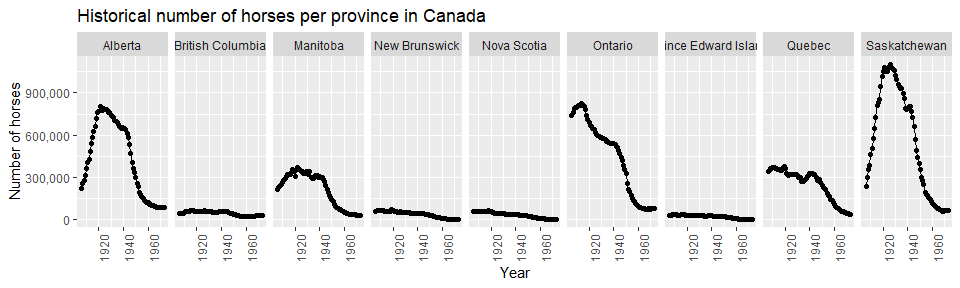
\includegraphics{hist_horse_pop_files/figure-latex/plot horses-1.pdf}

We can see from the visualisation above that Ontario, Saskatchewan and
Alberta have had the highest horse populations in Canada. All provinces
have had a decline in horse populations since 1940. This is likely due
to the rebound of the Canadian automotive industry after the Great
Depression and the Second World War. An interesting follow-up
visualization would be car sales per year for each Province over the
time period visualised above to further support this hypothesis.

Next we look at the range of the number horses for each provinces at any
time point between 1906 - 1973:

\begin{table}

\caption{\label{tab:max horse table}Table 1. This is the horse population in Canada}
\centering
\begin{tabular}[t]{l|r|r}
\hline
Province & Maximum & Minimum\\
\hline
Alberta & 806200 & 87000\\
\hline
British Columbia & 65200 & 22500\\
\hline
Manitoba & 370800 & 31000\\
\hline
New Brunswick & 71000 & 3200\\
\hline
Nova Scotia & 64500 & 3600\\
\hline
Ontario & 822300 & 75400\\
\hline
Prince Edward Island & 36700 & 2200\\
\hline
Quebec & 378800 & 39000\\
\hline
Saskatchewan & 1104300 & 58000\\
\hline
\end{tabular}
\end{table}

Below we zoom in and look at the province of Alberta:

\begin{figure}

{\centering 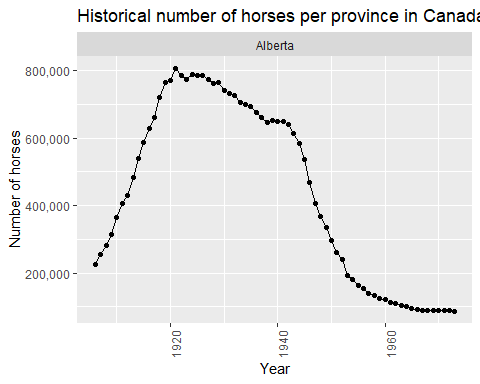
\includegraphics{hist_horse_pop_files/figure-latex/plot province-1} 

}

\caption{figure 2. horses per province}\label{fig:plot province}
\end{figure}

\hypertarget{reading-the-saved-plot}{%
\subsection{reading the saved plot}\label{reading-the-saved-plot}}

\begin{center}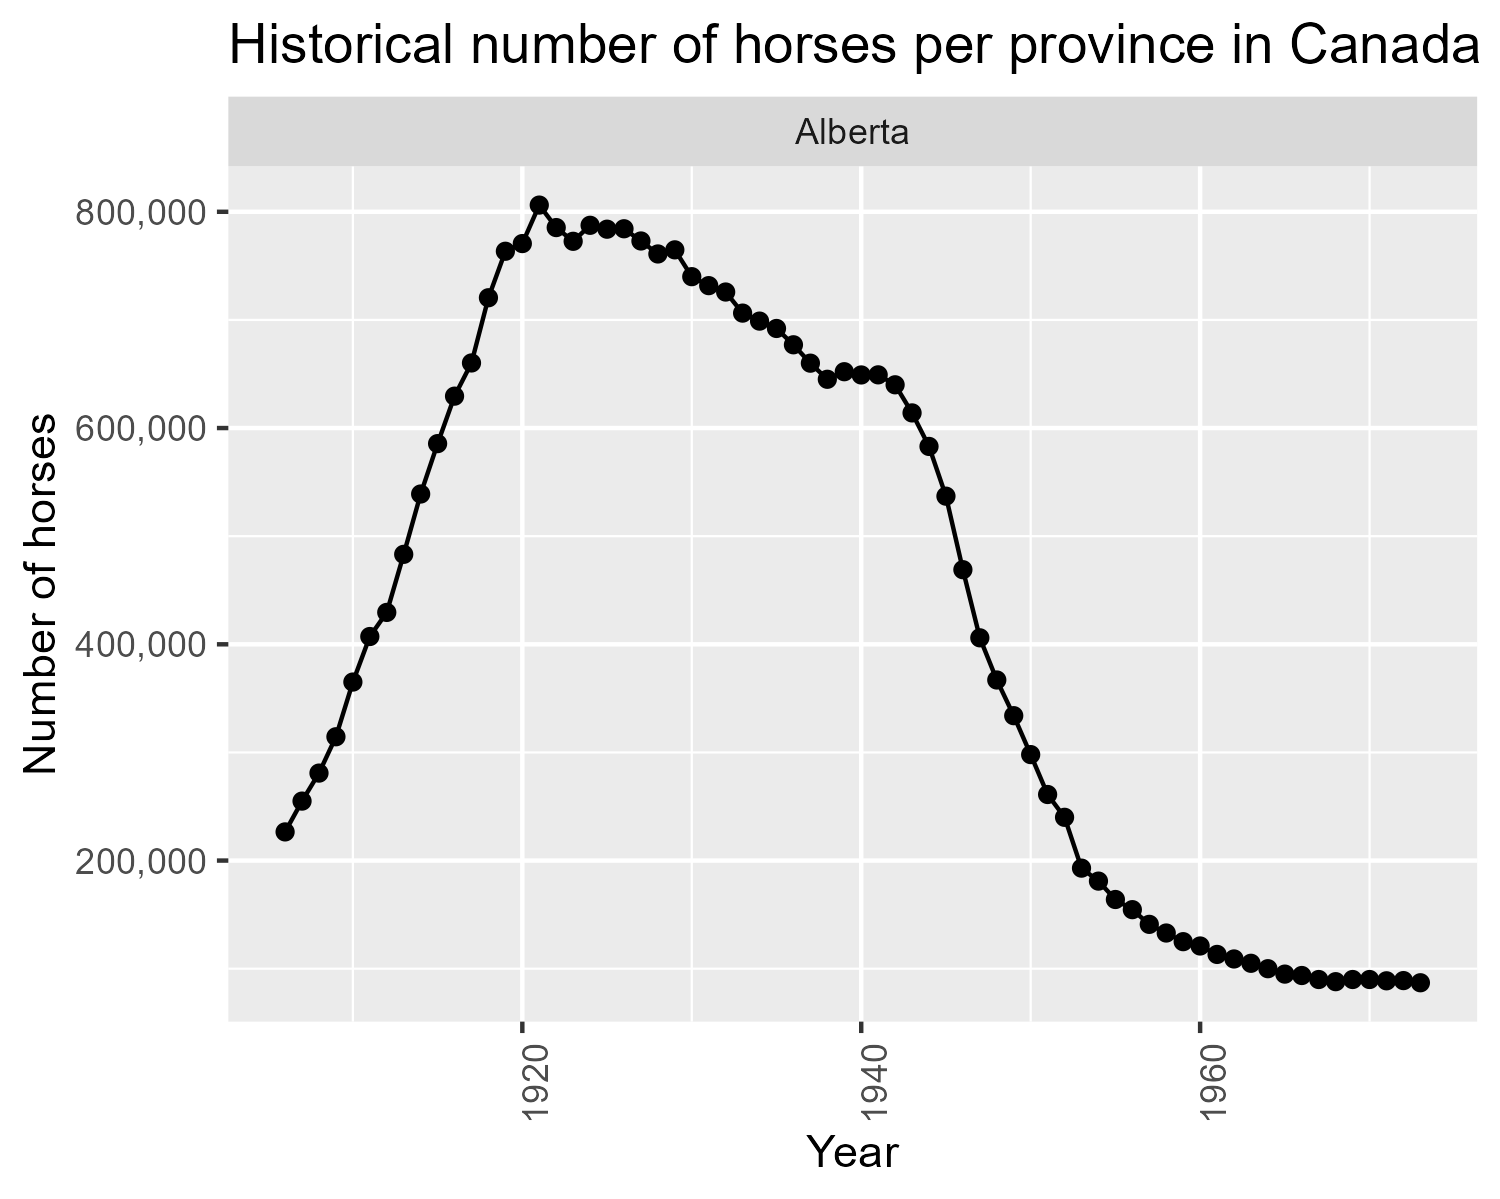
\includegraphics[width=0.4\linewidth,height=0.4\textheight]{province_plot} \end{center}

\hypertarget{references}{%
\subsection*{References}\label{references}}
\addcontentsline{toc}{subsection}{References}

\hypertarget{refs}{}
\begin{CSLReferences}{1}{0}
\leavevmode\vadjust pre{\hypertarget{ref-tidy}{}}%
Wickham, Hadley, Mara Averick, Jennifer Bryan, Winston Chang, Lucy
D'Agostino McGowan, Romain François, Garrett Grolemund, et al. 2019.
{``Welcome to the {tidyverse}.''} \emph{Journal of Open Source Software}
4 (43): 1686. \url{https://doi.org/10.21105/joss.01686}.

\end{CSLReferences}

\end{document}
